%%% template.tex
%%%
%%% This LaTeX source document can be used as the basis for your technical
%%% paper or abstract.

%%% The parameter to the ``documentclass'' command is very important.
%%% - use ``review'' for content submitted for review.
%%% - use ``preprint'' for accepted content you are making available.
%%% - use ``tog'' for technical papers accepted to the TOG journal and
%%%   for presentation at the SIGGRAPH or SIGGRAPH Asia conference.
%%% - use ``conference'' for final content accepted to a sponsored event
%%%   (hint: If you don't know, you should use ``conference.'')

\documentclass[review]{acmsiggraph}
\usepackage{amsmath}
\usepackage{amssymb}
\usepackage{wasysym}
\usepackage[scaled=.92]{helvet}
\usepackage{times}
\usepackage{graphicx}
\usepackage{parskip}
\usepackage{url}
\usepackage[labelfont=bf,textfont=it]{caption}
\usepackage{color}
\usepackage{algorithm}
\usepackage{algorithmic}
\usepackage{enumitem}
\usepackage{authblk}

%----------------------------------------------------------------------------
%----------------------------------------------------------------------------
\definecolor{AdamColor}{rgb}{0,0,0.7}
\definecolor{BenColor}{rgb}{0,0.7,0}
\definecolor{tamarColor}{rgb}{0.8,0,0.8}
\definecolor{JoshColor}{rgb}{0.0,0.7,0.8}
\newcommand{\mycomment}[1]{}
\newcommand{\adam}[1]{{\color{AdamColor} #1}}
\newcommand{\ben}[1]{{\color{BenColor} #1}}
\definecolor{nilsCol}{rgb}{0.85,0.35,0.25}
\newcommand{\Nils}[1]{\textcolor{nilsCol}{#1}}
\newcommand{\tamar}[1]{\textcolor{tamarColor}{#1}}
\newcommand{\josh}[1]{\textcolor{JoshColor}{#1}}
% for final
%\newcommand{\adam}[1]{{#1}}
%\newcommand{\Nils}[1]{{#1}}

%\let\shortcite=\cite
%\newcommand{\shortcite}[1]{\cite{#1}}
\newcommand{\etal}{and colleagues}
\newcommand{\Mueller}{M\"uller~}
\newcommand{\BM}[1]{\B{#1}}
%\newcommand{\B}[1]{\mbox{\boldmath$#1$}}
%\newcommand{\B}[1]{\textbf{\textit{#1}}}
\newcommand{\B}[1]{\mathit{\mathbf{#1}}}
\newcommand{\Per}{\%}
\newcommand{\Unit}[1]{{\mbox{$\,\mathrm{#1}$}}}
\newcommand{\Snit}[1]{{\mbox{\small$\mathrm{#1}$}}}
\newcommand{\Tr}[1]{\mathrm{Tr}\left(#1\right)}
\newcommand{\sign}[1]{\mathrm{sign}\left(#1\right)}
\newcommand{\Hz}{\Unit{Hz}}
\newcommand{\MHz}{\Unit{MHz}}
\newcommand{\GHz}{\Unit{GHz}}
\newcommand{\Sec}{\Unit{sec}}
\newcommand{\SPF}{\Unit{sec/frame}}
\newcommand{\Min}{\Unit{min}}
\newcommand{\Max}{\Unit{max}}
\newcommand{\M}{\Unit{m}}
\newcommand{\Nab}{\B{\nabla}}
\newcommand{\TP}{^\mathsf{T}}

\newcommand{\Dist}{\mbox{dist}}

\newcommand{\figureTopBot}[1]{
  \begin{figure}[!tb]{\sloppy #1}\end{figure}
}

\newcommand{\figureTop}[1]{
  \begin{figure}[!t]{\sloppy #1}\end{figure}
}
 
\newcommand{\figureBot}[1]{
  \begin{figure}[!b]{\sloppy #1}\end{figure}
}

\newcommand{\figureWideTop}[1]{
  \begin{figure*}[!t]{\sloppy #1}\end{figure*}
}

\newcommand{\figureWideBot}[1]{
  \begin{figure*}[!b]{\sloppy #1}\end{figure*}
}

\newcommand{\eqAlgn}{\!\!&\!\!}

\newcommand{\Eref}[1]{Equation~(\ref{#1})}
\newcommand{\Erefs}[2]{Equations~(\ref{#1}) and (\ref{#2})}
\newcommand{\eref}[1]{Equation~(\ref{#1})}
\newcommand{\erefs}[2]{Equations~(\ref{#1}) and (\ref{#2})}
\newcommand{\Sref}[1]{Section~\ref{#1}}
\newcommand{\sref}[1]{Section~\ref{#1}}
\newcommand{\srefs}[2]{Sections~\ref{#1} and~\ref{#2}}
\newcommand{\fref}[1]{Figure~\ref{#1}}
\newcommand{\frefAND}[2]{Figures~\ref{#1} and~\ref{#2}}
\newcommand{\frefs}[2]{Figures~\ref{#1} and~\ref{#2}}
\newcommand{\frefss}[3]{Figures~\ref{#1}, \ref{#2}, and~\ref{#3}}
\newcommand{\frefsss}[4]{Figures~\ref{#1}, \ref{#2}, \ref{#3}, and~\ref{#4}}
\newcommand{\Fref}[1]{Figure~\ref{#1}}
\newcommand{\Frefs}[2]{Figures~\ref{#1} and~\ref{#2}}
\newcommand{\Frefss}[3]{Figures~\ref{#1}, \ref{#2}, and~\ref{#3}}
\newcommand{\Frefsss}[4]{Figures~\ref{#1}, \ref{#2}, \ref{#3}, and~\ref{#4}}
\newcommand{\tref}[1]{Table~\ref{#1}}

\renewcommand{\labelenumi}{\arabic{enumi}.}
\renewcommand{\labelenumii}{\alph{enumii}.}
\renewcommand{\labelenumiii}{\roman{enumiii}.}

\newenvironment{algstep}{%
  \begin{enumerate}%
    \setlength{\itemsep}{0in}%
    \setlength{\partopsep}{0in}%
    \setlength{\topsep}{0in}%
}{\end{enumerate}}

%----------------------------------------------------------------------------
%----------------------------------------------------------------------------

%%% Make the ``BibTeX'' word pretty...

\def\BibTeX{{\rm B\kern-.05em{\sc i\kern-.025em b}\kern-.08em
    T\kern-.1667em\lower.7ex\hbox{E}\kern-.125emX}}

%%% Used by the ``review'' variation; the online ID will be printed on 
%%% every page of the content.

\TOGonlineid{70}

%%% Used by the ``preprint'' variation.

\TOGvolume{0}
\TOGnumber{0}

\title{Ductile Fracture for Clustered Shape Matching}
\author[*]{Ben Jones}
\author[**]{Joshua A. Levine}
\author[***]{Tamar Shinar}
\author[*]{Adam W. Bargteil}
\affil[*]{University of Utah}
\affil[**]{Clemson University}
\affil[***]{University of California, Riverside}
\pdfauthor{}

\keywords{Shape Matching, Ductile Fracture}

\begin{document}

%%% This is the ``teaser'' command, which puts an figure, centered, below 
%%% the title and author information, and above the body of the content.

 \teaser{
   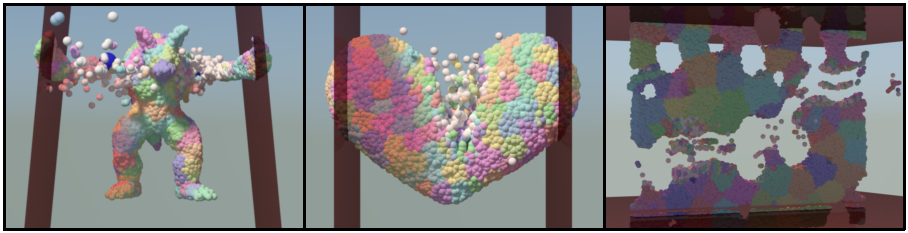
\includegraphics[width=\linewidth]{Figures/teaser}
   \caption{Left: An armadillo is tortured by being torn apart by the arms while being fired upon by spherical projectiles.  Center: A heartbreaking example.  Right: Tearing a slice of swiss cheese.}
   \label{fig:teaser}
 }

\maketitle

\begin{abstract}
In this paper, we incorporate ductile fracture into the clustered shape matching simulation framework
for deformable bodies, thus filling a gap in the shape matching literature.  The resulting approach is fast,
versatile, and simple to implement.
\end{abstract}

\begin{CRcatlist}
  \CRcat{I.3.7}{Computer Graphics}{Three-Dimensional Graphics and Realism}{Animation};
  \CRcat{I.6.8}{Simulation and Modeling}{Types of Simulation}{Animation}.
\end{CRcatlist}

\keywordlist

%% Required for all content. 

\copyrightspace

\section{Introduction}\label{sec:Introduction}
{\em Shape matching} is a geometrically motivated technique for animating deformable bodies introduced
a decade ago by \Mueller and colleagues~\shortcite{Mueller:2005:MDB}.
\fref{fig:shapematching} summarizes the approach.
In their seminal work, \Mueller and colleagues~\shortcite{Mueller:2005:MDB} introduced a simple plasticity
model and, in follow up work, Rivers and James~\shortcite{Rivers:2007:FFL}
incorporated a simple fracture model.  However, ductile fracture has not yet been addressed in the
shape matching literature.

\begin{figure*}
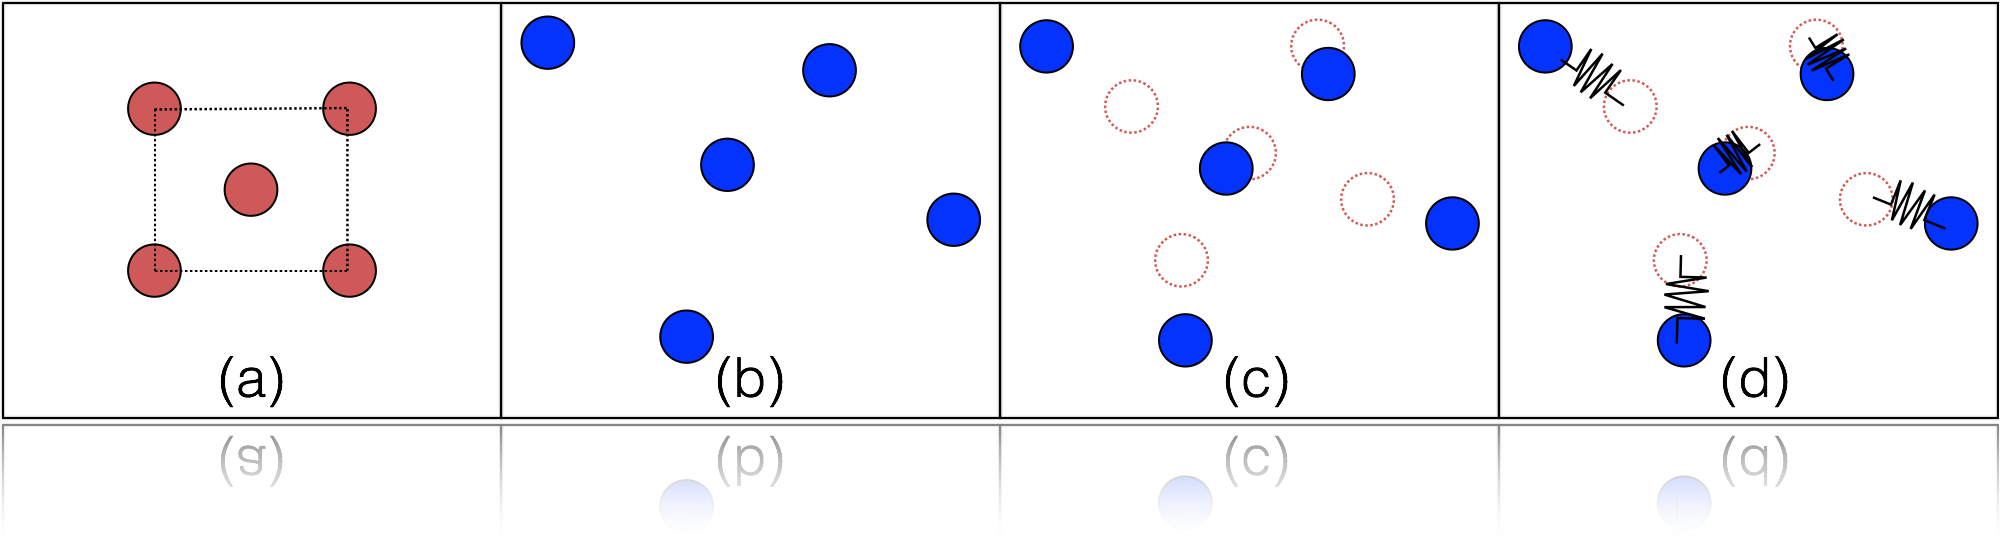
\includegraphics[width=\linewidth]{Figures/shapematching.png}
\caption{Shape Matching Overview: (a) An object (here, a square) is sampled with particles, $p_i$, to get rest positions, $\B{r}_i$.  
(b) As particles are subjected to external forces and constraints, their positions, $\B{x}_i$, are updated in world space.  
(c)  The best-fitting rigid transformation of the particles' rest positions, $\B{r}_i$, 
to their world positions, $\B{x}_i$ is computed.  The dotted red circles are the {\em goal} positions, $\B{g}_i$.  
(d) Hookean springs pull the world positions toward the goal positions.}
\label{fig:shapematching}
\end{figure*}

%In this paper, we incorporate ductile fracture into the clustered shape matching simulation framework
%for deformable bodies, thus filling a gap in the shape matching literature. 
In this paper, we enable the animation of ductile fracture 
by incorporating plasticity and fracture models into the clustered shape matching framework.
Our models are inspired by finite element approaches to animating deformable bodies, but are adapted to 
clustered shape matching.
Specifically, inspired by the work of Irving and colleagues~\shortcite{Irving:2004:IFE} and Bargteil and 
colleagues~\shortcite{Bargteil:2007:AFE}, we introduce a multiplicative plasticity model that incorporates
yield stress, flow rate, and work hardening.  Inspired by the work of O'Brien and colleagues~\shortcite{Obrien:1999:GMA,Obrien:2002:GMA},
we introduce a cluster-based fracture approach that splits individual clusters along the plane orthogonal to the direction the 
cluster is most stretched.
Taken together these contributions allow animation of ductile fracture in the clustered shape matching framework, as demonstrated
in~\fref{fig:teaser}.

\section{Related Work}
The geometrically motivated shape matching approach was introduced by \Mueller and 
colleagues~\shortcite{Mueller:2005:MDB}, who demonstrated impressive results and 
described the key advantages of the approach: efficiency, stability, and controllability.
Given these advantages, shape matching is especially appealing in interactive animation contexts such as
video games.  The authors also introduced several extensions including linear and quadratic deformations 
(in addition to rigid deformations), cluster-based deformation, and plasticity.  

Two years later, Rivers and James~\shortcite{Rivers:2007:FFL} introduced lattice-based shape matching,
which used a set of hierarchical lattices to define the shape matching clusters.  They took advantage
of the regular structure of the lattices to achieve extremely high performance.  They also incorporated a 
simple fracture model that removed over-extended links in the lattice.  

Despite impressive results and substantial promise,
the shape matching framework has been largely disregarded by the research community in favor of position-based
dynamics~\cite{Mueller:2007:PBD,Bender:2013:PBM,Bender:2014:ASO,Macklin:2014:UPP}.  One notable exception is
the work of Bargteil and Jones~\shortcite{Bargteil:2014:SLF}, which incorporated strain-limiting into clustered shape matching
and pointed out several advantages of shape matching over position-based dynamics.
We incorporate our ductile fracture approach into their open-source framework.

Ductile fracture is distinguished from brittle fracture by the inclusion of plastic deformation.  Materials undergoing ductile
fracture (e.g. play dough) appear to {\em tear}, while brittle materials (e.g. glass) appear to {\em shatter}.  Most
real-world materials demonstrate some amount of plastic deformation during failure, so purely brittle models have fairly limited
application in computer animation.  
Both plasticity and fracture
were first demonstrated in computer animation by the pioneering work of Terzopoulos and Fleischer~\shortcite{Terzopoulos:1988:MID}; 
however, it was O'Brien and colleagues~\shortcite{Obrien:2002:GMA}
who first combined these phenomena to animate ductile fracture.  Since that time, plasticity and fracture have
remained very active research areas in computer animation and a thorough review is beyond the scope of this short paper.
\mycomment{\adam{in part this is because I am lazy, does anyone think it would be important?}
\josh{I think the review would only be important if we were able to draw
a conclusion like ``the most promising way to apply it in the context of
csm is blah...'', or some other general trend regarding it that's
applicable in this context}}

Our approach 
to fracture closely resembles that of O'Brien and colleagues~\shortcite{Obrien:1999:GMA,Obrien:2002:GMA}; however, instead of splitting tetrahedra,
we split shape matching clusters.  Our plasticity model closely resembles that of Bargteil and colleagues~\shortcite{Bargteil:2007:AFE}, except that
we apply it to shape matching clusters instead of individual tetrahedra and make no particular effort to ensure that plastic deformation does not
lead to instability, i.e.~we do not update clusters to ensure well-conditioned matrices as done by, for example, Jones and colleagues~\shortcite{Jones:2014:DEF}.

\section{Methods}
For completeness and readability, we first briefly review the shape matching approach of \Mueller and colleagues~\shortcite{Mueller:2005:MDB} before
introducing our plasticity and fracture models.  Finally we briefly discuss our approaches to sampling and clustering.
\subsection{Shape Matching}
\label{sec:ShapeMatching}
In the shape matching framework
objects are discretized into a set of particles, $p_i\in\mathcal{P}$, with masses, $m_i$, and rest positions, $\B{r}_i$, 
that follow a path, $\B{x}_i(t)$, in world-space through time.  
Shape matching takes its name from the fact that, each frame, we match the rest shape to 
the deformed shape by finding
the least-squares best-fit rigid transformation from the rest pose
to the current deformed pose by
solving for the rotation matrix, $\B{R}$, and translation
vector, $\B{x}_{cm}-\B{r}_{cm}$, that minimizes
\begin{equation}
\label{eq:sm}
\sum_i m_i \| \B{R}\left(\B{r}_i - \B{r}_{cm}\right)-\left(\B{x}_i-\B{x}_{cm}\right)\|^2.
\end{equation}
The best translation is given by the center-of-mass in the rest and world space.  
Computing the rotation, $\B{R}$, is more involved.  
We first compute the least-squares best-fit linear deformation gradient, $\B{F}$.
Specifically, we seek the $\B{F}$ that minimizes
\begin{equation}
\sum_i m_i \| \B{F}\left(\B{r}_i - \B{r}_{cm}\right)-\left(\B{x}_i-\B{x}_{cm}\right)\|^2.
\end{equation}
Setting the derivative with respect to $\B{F}$ to $0$ and re-arranging terms we arrive at
\begin{equation}
\label{eq:defgrad}
\B{F} = \left(\sum_i m_i \B{O}(\B{x}_i,\B{r}_i)\right)\left(\sum_im_i\B{O}(\B{r}_i,\B{r}_i)\right)^{-1} = \B{A}_{xr}\B{A}_{rr}^{-1},
\end{equation}
where $\B{O}(\cdot,\cdot)$ is the outer product matrix
\begin{equation}
\B{O}(\B{a}_i,\B{b}_i) = \left(\B{a}_i-\B{a}_{cm}\right)\left(\B{b}_{i}-\B{b}_{cm}\right)^T,
\end{equation}
and $\B{A}_{**}$ is a convenient shorthand.
%\begin{align}
%\B{F} = &\left(\sum_i m_i\left(\B{x}_{i}-\B{x}_{cm}\right)\left(\B{r}_{i}-\B{r}_{cm}\right)^T\right)\notag\\
%&\left(\sum_i m_i\left(\B{r}_{i}-\B{r}_{cm}\right)\left(\B{r}_{i}-\B{r}_{cm}\right)^T\right)^{-1},
%\end{align}
%and $m_i$ is the mass of $p_i$. 
We then compute $\B{R}$ using the polar decomposition,
\begin{equation}
\label{eq:decomp}
\B{F} = \B{R}\B{S} = \left(\B{UV}^T\right)\left(\B{V\Sigma V}^T\right)
\end{equation}
where $\B{S}=\B{V\Sigma V}^T$ is a symmetric matrix and $\B{U\Sigma V}^T$ is the singular value decomposition (SVD) of $\B{F}$.
While several researchers (e.g.~\cite{Rivers:2007:FFL}) have pointed out that polar decompositions can be computed faster than the SVD,
especially when warm started, we use the SVD for its robustness and for our plasticity and fracture models 
(see~\srefs{sec:Plasticity}{sec:Fracture}).  
We also note that we compute the polar decomposition of $\B{F}$, not
the left matrix ($\B{A}_{xr}$)
%($\sum_im_i\B{O}(\B{x}_i,\B{r}_i)$) 
as done by \Mueller and colleagues~\shortcite{Mueller:2005:MDB}.  This modification
is particularly important if the distribution of mass in the cluster is non-uniform and $\B{F}$ is not a pure rotation.

Given $\B{R}$ and $\B{x}_{cm}-\B{r}_{cm}$, we define goal positions, $\B{g}_i$, as
\begin{equation}
\B{g}_i = \B{R}\left(\B{r}_i-\B{r}_{cm}\right)+\B{x}_{cm}.
\end{equation}
Hookean springs are then used to define forces that move the particles toward the goal positions.

\paragraph{Clustered Shape Matching}
Handling multiple clusters is straightforward.  When computing a particle's contribution to 
cluster quantities, we divide the particle's mass by the number of clusters it belongs to,
essentially replacing $m_i$ with $m_i/n_i$ in equations \eqref{eq:sm}-\eqref{eq:defgrad} 
and when computing cluster mass and center-of-mass.
Specifically, if particle $p_i$ belongs
to $n_i$ clusters, then the center-of-mass of cluster $c$, $\B{x}_{cm,c}$, is
\begin{equation}
\B{x}_{cm,c} = \frac{\sum_{p_i\in\mathcal{P}_c}(m_i/n_i)\B{x_i}}{\sum_{p_i\in\mathcal{P}_c}(m_i/n_i)},
\end{equation}
where $\mathcal{P}_c$ is the set of particles in cluster $c$.
Furthermore, when computing the goal position, $\B{g}_i$, for a particle we perform a simple
average of the goal positions given by each cluster it is a part of.  That is,
\begin{equation}
\B{g}_i = \frac{1}{n_i} \sum_c \B{g}_{i,c},
\end{equation}
where $\B{g}_{i,c}$ is the goal position for particle $p_i$ in cluster $c$.

\paragraph{Strain Limiting}
To maintain stability we adopt the strain limiting approach advocated by Bargteil and Jones~\shortcite{Bargteil:2014:SLF}.
However, in the presence of plastic deformation (see~\sref{sec:Plasticity}) we typically increase the maximum allowed stretch ($\gamma$ in
their paper) to avoid instabilities when clusters disagree about the current rest shape.

\subsection{Plasticity}
\label{sec:Plasticity}
To accommodate plastic deformation we store and update an additional matrix, $\B{F}^p_c$, for each cluster, $c$.
For readability we drop the subscript, but the following is computed for each cluster.
We then compute the elastic part of the deformation gradient
\begin{equation}
\B{F}^e = \B{F} \left(\B{F}^p\right)^{-1},
\end{equation}
where $\B{F}$ is given by~\eref{eq:defgrad}.  We then decompose $\B{F}^e$ in~\eref{eq:decomp}.

$\B{F}^p$ is initialized to the identity, $\B{I}$.  Then each timestep we compute the volume preserving part 
of the diagonalized $\B{F}^e$,
\begin{equation}
\B{F}^* = \det(\B{\Sigma}^e)^{-1/3}\B{\Sigma}^e.
\end{equation}
We then compare
\begin{equation}
\|\B{F}^* - \B{I}\|_F
\end{equation}
to a plastic yield threshold, $\lambda$, where $\|\cdot\|_F$ is the Frobenius norm.  If the threshold
is not exceeded $\B{F}^p$ remains unchanged.  Otherwise we update $\B{F}^p$ by
\begin{equation}
\B{F}^p_{new} = \left(\B{F}^*\right)^\gamma\B{V}\B{F}^p_{old},
\end{equation}
where $\B{V}$ is the matrix of right singular vectors in~\eref{eq:decomp} and $\gamma$ is given by
\begin{equation}
\gamma = \min\left(\frac{\nu * \|\B{F}^* - \B{I}\|_F - \lambda - K\alpha}{\|\B{F}^* - \B{I}\|_F},1\right),
\end{equation}
where $\nu$ and $K$ are user-given flow rate and work hardening/softening constant, respectively, 
and $\alpha$ is a measure of cumulative stress that is initialized to zero and then updated by
\begin{equation}
\dot{\alpha} = \|\B{F}^e-\B{I}\|_F.
\end{equation}
We do not apply additional left-hand rotations when computing $\B{F}^p_{new}$ as these would be discarded during
the decomposition in~\eref{eq:decomp}.


\subsection{Fracture}
\label{sec:Fracture}
To model fracture, we allow shape matching clusters to split into two clusters.  Each timestep, for each cluster,
we compare the largest singular value, $\Sigma_{\max}$, computed in~\eref{eq:decomp}, to a toughness, $\tau_c$, which
can vary between clusters.  
If $\Sigma_{\max} > \tau_c$ then the cluster is added to a priority queue with priority $\Sigma_{\max} - \tau_c$.  We also
record the corresponding right singular vector $\B{V}_{\max}$.  The fracture process occurs 
at the end of the timestep, after computing dynamics.  We iteratively remove
clusters from the priority queue and, if the $\Sigma_{\max}$ still exceeds $\tau_c$, we split the cluster into two clusters
as follows.

We assume that the fracture surface is defined by the plane that passes through the center of mass of the 
cluster, $\B{x}_{cm,c}$, and is orthogonal to the singular vector $\B{V}_{\max}$.  Particles on the positive%\adam{?}
 side of this plane are removed from the cluster and added to a new cluster.  Additionally, we remove particles 
from any other cluster, $d$, where the center of mass, $\B{x}_{cm,d}$ is on the other side of the fracture surface.
That is if, for particle $p_i$,
\begin{equation}
\sign{\left(\B{x}_i-\B{x}_{cm,c}\right)\cdot \B{V}_{\max}} \mathrel{!}=
\sign{\left(\B{x}_{cm,d}-\B{x}_{cm,c}\right)\cdot \B{V}_{\max}}
\end{equation}
particle $p_i$ is removed from cluster $d$.  We then update the properties of the affected clusters.
The plasticity variables, $\B{F}^p$ and $\alpha$, are copied from the fractured cluster to the new cluster.
For every cluster that undergoes a membership change, we update the mass, $m_c$; the 
rest and world center of mass, $\B{r}_{cm,c}$ and $\B{x}_{cm,c}$; the cluster width (see~\cite{Bargteil:2014:SLF});
and the stored matrix, $\B{A}_{rr}^{-1}$.  To handle potentially degenerate clusters, we compute $\B{A}_{rr}^{-1}$
through the pseudoinverse.  If, when computing the pseudoinverse, any of the singular values are thresholded,
we set $\B{F}_c^p = \B{I}$.  We also update particle-to-cluster maps and $n_i$ for affected particles.

Because cluster membership may have changed due to the fracturing of a different cluster, we verify that 
$\Sigma_{\max} > \tau_c$ before fracturing and also recompute $\B{V}_{\max}$.

\subsection{Sampling and Clustering}

Both the distribution of particles that model and object as well as the
clustering of particles affect the resulting simulation.  We
experimented with both grid-based and blue noise sampling and
preferred the results from blue noise over the highly structured grid-based sampling.
Our blue noise sampler is based on Bridson's fast Poisson disk
sampling~\cite{Bridson:2007:FPD}.  In both cases, for objects whose
boundary is an arbitrary manifold, we simply sample particles within
the bounding box of the object and discard particles outside
the surface.

The selection of clusters affects the effective distribution of mass 
within the object.  Bargteil and Jones~\shortcite{Bargteil:2014:SLF}
allowed the user to select a cluster width, $w$, and then
chose cluster centers randomly from the simulation particles until every particle
was in at least one cluster.  They complained that this approach led
to a highly non-uniform distribution of mass over the object.  
To mitigate this artifact, we use a variant of the
well know $k$-means algorithm.  The user specifies both the
number of clusters, $n$, and the cluster width, $w$.
We initialize $n$ clusters as randomly selected seed particles.
Particles are then placed into the cluster to which they are closest.
We then iteratively compute the center of mass for each cluster, and
redistribute the particles into the clusters based on distance to the
nearest center of mass.  This process iterates until 
convergence.  Finally, we include particle $p_i$ within any cluster, $c$,
such that the distance between $p_i$ and the cluster's center
of mass, $\B{r}_{cm,c}$, is less than $w$.  That is
\begin{equation}
p_i\in\mathcal{P}_c \iff \|\B{r}_i-\B{r}_{cm,c}\| < w.
\end{equation}

%\josh{what else needs to be said here?}

\section{Results and Discussion}
\begin{figure}[h!]
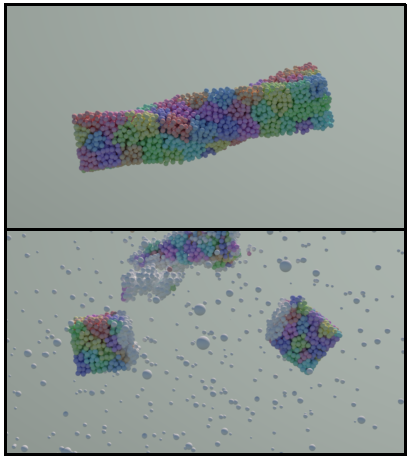
\includegraphics[width=\linewidth]{Figures/TwistedBar}
\caption{A bar is twisted and then the clamps are released.  Top: A tough plastic bar does not fracture.  Bottom: The bar fractures before the clamps are released.}
\label{fig:twistedbar}
\end{figure}

\begin{figure}
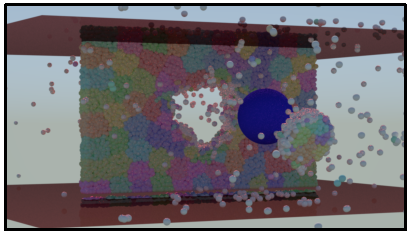
\includegraphics[width=\linewidth]{Figures/projectile}
\caption{A projectile is fired through a thin sheet of material.}
\label{fig:projectile}
\end{figure}

We have used our method to animate a number of examples of ductile fracture.  Timing results
taken on a Macbook Pro with a 2.4GHz Intel i5 processor.
are given in table~\tref{table:timing}.
In all particle renderings, particle color is used to indicate the nearest cluster center.  
We stress that clusters overlap and that particles typically belong to more than one cluster.

\begin{table*}
\begin{center}
\caption{Timing results in ms per frame taken on a Macbook Pro with a 2.4Ghz Intel i5 processor.}
\label{table:timing}
\begin{tabular}{|l|l|l|l|l|l|}
\hline
example & \# particles & dynamics & fracture & plasticity & total\\
\hline
armadillo & 20115 & 24  & $<$ 1 & 38 & 65\\
twisted bar & 5317 & 7 & $<$ 1  & 0 & 7\\
twisted bar with fracture & 5317 & 11  & $<$ 1 & 2.5 & 15 \\
projectile & 5325 & 29 & $<$ 1 & 24 & 57\\
broken heart & 20132 & 23 & $<$ 1 & 15 & 41\\
swiss cheese & 25032 & 27 & $<$ 1 & 39 & 69 \\
\hline
\end{tabular}
\end{center}
\end{table*}

In our first example, an armadillo is tortured by simultaneously pulling on and firing
canonballs at its arms (see~\fref{fig:teaser}).
Our second example is more didactic; a simple bar is twisted (see~\fref{fig:twistedbar}).  First we demonstrate 
plastic deformation, which allows the bar to maintain its twisted shape, then we enable fracture. 
In our thrid example a projectile is fired through a thin sheet of material (see~\fref{fig:projectile}).  
In our heartbreaking fourth example a complex shape is pulled apart (see~\fref{fig:teaser}).  The complex shape determines
where the tear begins and how it propogates.  Similarly, in our final example the holes in a 
slice of swiss cheese determine how the model is torn (see~\fref{fig:teaser}).

%Timing stuff: make a table shell and I can fill it in.  Probably makes sense to do average time/frame of simulation (shape matching/strain limiting), fracture, plasticity.

%One view of clustered shape matching is that there are far fewer integration units than degrees of freedom compared to
%fem.  This makes sense for computer graphics applications where degrees of freedom correspond lead to visual detail 
%while integrations units lead to computational cost.

%We could compare our approaches to plasticity and fracture to Irving2004,Barteil2007 and O'Brien1999. 

\paragraph{Limitations and Future Work}
%\ben{limitation: variable framerate, fracture can slow down the simulation IMMENSELY in current implementation}
Our approach has a number of limitations that provide ample potential for future work in clustered shape matching.
One limitation of our implementation is that we only handle simple collision geometry and do not handle self-collisions.
More complicated collision geometry should be easily handled using well-established signed-distance field approaches~\cite{Guendelman:2003:NRB}.
Handling self-collisions would require further research; the sphere-packing approach of Budsberg and colleagues~\shortcite{Budsberg:2014:EPD}
seems particularly promising.  
Another limitation of our current implementation is that the computational cost is somewhat unpredictable; many fractures occuring at once
can have a very significant impact on performance.  In the future it would be interesting to explore asynchronous fracturing
where, instead of emptying the priority queue every timestep, it is processed as computational resources allow.

Like many fracture methods in computer animation, we do not have a good solution to generating fractured
geometry.  Like previous work~\cite{Mueller:2005:MDB,Rivers:2007:FFL}, we can embed a high-resolution 
render mesh for unbreakable objects, but creating new geometry when fracture occurs is more difficult.  
Currently we use an off-the-shelf particle skinning tool~\cite{Bhattacharya:2015:ALM} to skin the simulation particles.
This approach suffers two major drawbacks: the results are low-resolution and the fracture surfaces are overly smooth.
One approach to generating fracture geometry is to simply render the simulation geometry and increase the resolution 
where fracture occurs~\cite{Obrien:1999:GMA,Obrien:2002:GMA}.  The simulation geometry can can later be 
coarsened to improve computational efficiency~\cite{Pfaff:2014:ATC}.  This approach leads to
somewhat unpredictable costs and is, at present, too slow for the interactive applications where shape matching excels.
Levine and colleagues~\shortcite{Levine:2014:APP} suggested a number of other techniques for generating fracture geometry
for spring-mass systems that may be applicable in our interactive context.  Exploring these ideas is an interesting avenue 
for future work.

Our blue-noise sampling and k-means clustering improve upon the regular grids and
randomized clusters of Bargteil and Jones~\shortcite{Bargteil:2014:SLF} and are effective for our purposes,
but better approaches certainly exist.  In particular, it would be interesting to explore adaptive sampling
so that computational resources can be focused on interesting areas of the object.  It would also be interesting
to consider adaptive and hierarchical clustering techniques; the hierarchical lattices of Rivers and James~\cite{Rivers:2007:FFL}
clearly improved performance and artistic directability.  Relatedly, we do not currently place any bounds on the minimum
number of particles in a cluster.  Consequently our results contain many one-particle clusters, which results in a 
``particle spray'' look that may be objectionable in some contexts.

The biggest limitation of our approach is a lack of theoretical underpinnings for the clustered shape matching
framework; we do not yet have any mathematical tools to analyze the approach.  We do not really understand
how the method behaves as particle counts or timesteps decrease or as the cluster size or number of clusters change.
This limitation does not mean the approach is not useful.  After all, the finite element method was in use
for decades before a mathematical framework was developed to analyze its properties.  In a similar way,
even though we do not have a deep understanding of the approach, the clustered shape-matching framework, with its
relatively large particle-to-cluster ratio,
is particularly useful for graphical applications, especially interactive applications, where visual detail
and computational efficiency are of paramount importance.



\section*{Acknowledgements}
Removed for anonymous review.

\bibliographystyle{acmsiggraph}
\bibliography{csm}
\end{document}
